% !TEX root = ./sum1.tex
\section{Deterministic Model}

\subsection{Obtain Minimum Number of Rows to Cover Demand}

We are given a demand, for example, $(d_1, d_2, d_3, d_4, d_5, d_6) = (3,5,7,0,10,6)$, where $d_i$ indicates the number of group containing $i$ people. Suppose each group has to leave a seat to maintain social distancing with the adjacent groups. Regard the groups as items in the CSP, and rows as stocks to be cut.
With considering the social distancing, the size of each group should be treated as the actual size plus one. Then each row of seats should also add a dummy(virtual) seat for the same reason, and the number of all seats in each row is called the length of the row.

To find the minimum number of rows to satisfy the demand, we can formulate this problem as a cutting stock problem form and use the column generation method to obtain an approximate solution.

Similar to the concept of pattern in the CSP, let the $k$-th placing pattern of a line of seats with length $S$ into some of the $m$ group types be denoted as a vector $(t^k_1,t^k_2,\ldots,t^k_m)$. Here, $t^k_i$ represents the number of times group type $i$ is placed in the $k$-th placing pattern. For a pattern $(t^k_1,t^k_2,\ldots,t^k_m)$ to be feasible, it must satisfy: $\sum_{i=1}^m t^k_i s_i \leq S$, where $s_i$ is the size of group type $i$. Denote by $K$ the current number of placing patterns.


This problem is to decide how to place a total number of group type $i$ at least $g_i$ times, from all the available placing patterns, so that the total number of rows of seats used is minimized.

Immediately we have the master problem:

\[\begin{split}\mbox{min}\quad & \sum_{k \in K}^K x_{k}\\
 \mbox{s.t.} \quad & \sum_{k \in K}^K t_i^k x_k \geq d_i  \quad  \mbox{ for } i=1,\ldots,m \\
  & x_k \geq 0, \mbox{integer}\quad \mbox{for}~ k \in K,\ldots,K.\\
\end{split}\]

If $K$ includes all possible patterns, we can obtain the optimal solution by solving the corresponding IP. But it is clear that the patterns will be numerous, considering all possible patterns will be time-consuming.

Thus, we need to consider the linear relaxation of the master problem, and the optimal dual variable vector $\lambda$. Using $\lambda$ as the value assigned to each group type $i$, the next problem is to find a feasible pattern $(y_1,y_2,\ldots,y_m)$ that maximizes the product of $\lambda$ and $y$.


Then the corresponding sub-problem is:
\[\begin{split}\mbox{max}\quad & \sum_{i=1}^m \lambda_i y_{i}\\
        \mbox{s.t.} \quad & \sum_{i=1}^m w_i y_i \leq S  \\
        & y_i \geq 0, \mbox{integer}\quad \mbox{for}~ i=1,\ldots,m.\\
\end{split}\]

This is a knapsack problem, its solution will be used as an additional pattern in the master problem.
We should continue to add new pattern until all reduced costs are nonnegative. Then we have an optimal solution to the original linear programming problem.

But note that column generation method cannot gaurantee an optimal solution. If we want to reach the optimal solution, we should tackle with the integer formulation.

\begin{equation}
\begin{aligned}
\min \sum_{k \in K}^{K} y_{k} & \\
\sum_{k=1}^{K} x_{i k} & \geq d_{i} \quad i=1, \ldots, n \\
\sum_{i=1}^{n} a_{i} x_{i k} & \leq S y_{k} \quad k=1, \ldots, K \\
y_{k} & \in\{0,1\} \quad k=1, \ldots, K \\
x_{i k} & \geq 0 \text { and integer } i=1, \ldots, n ; k=1, \ldots, K
\end{aligned}
\end{equation}

$y_k =1$ if line $k$ is used and 0 otherwise, $x_{ik}$ is the number of times group $i$ is placed in row $k$, and $K$ is the upper bound on the number of the rows needed.

\subsection{Provide The Maximal Supply When Given Rows}\label{maximal_supply}

Let us review this problem in another way. In most cases where the number of rows is fixed, we hope to accommodate as many as people possible. That is, we should minimize the space loss.

% This can be illustrated from the following picture.
%
% \begin{figure}[h]%%图
% 	\centering  %插入的图片居中表示
% 	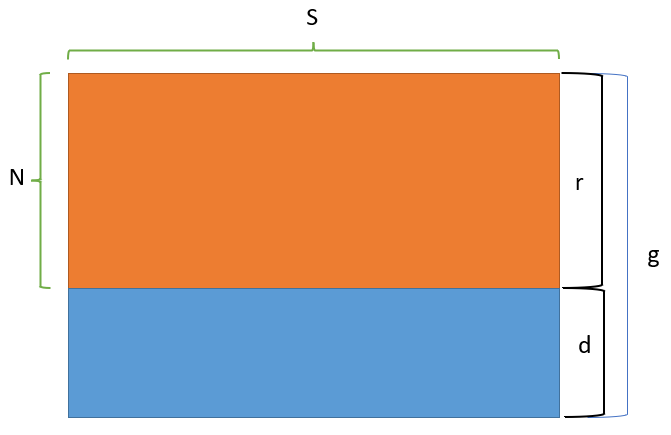
\includegraphics[width = 0.6\textwidth]{Figures/illu.png}  %插入的图,包括JPG,PNG,PDF,EPS等,放在源文件目录下
% 	\caption{The illustration for minimizing space loss}  %图片的名称
% 	\label{fig:illustration}   %标签,用作引用
% \end{figure}
%
% $N$: the number of given rows. $S$: the length of the line. $g$: total demand. $r$: remaining demand  $d$: discarded demand.

Then minimizing $NS - \sum_{i=1}^m r_i(s_i-1)$ equals to maximize $\sum_{i=1}^m r_i(s_i-1)$ and maximze $\sum_{i=1}^m (g_i - d_i)(s_i-1)$.

Notice that $\sum_{k=1}^K t_i^k x_k + d_i = g_i$, by substituting this equation we can obtain the objective function of the following master problem.

\begin{align}
(D) \quad \mbox{max}\quad & \sum_{k=1}^K(\sum_{i=1}^m (s_i-1)t_i^k) x_{k} \notag \\
\mbox{s.t.} \quad & \sum_{k=1}^K x_{k} \leq N \label{lambda1} \\
& \sum_{k=1}^K t_i^k x_k \leq g_i,\quad i=1,\ldots,m  \label{mu1} \\
& x_{k} \geq 0, \quad k = 1,\ldots,K \notag
\end{align}

Similarly, we consider the linear relaxation of the master problem and the optimal dual variable vector $\lambda,\mu$. Using $\lambda$ as the value assigned to the first constraint \eqref{lambda1} and $\mu$ to the second constraints \eqref{mu1}. This master problem is to find a feasible pattern $(t_1^{k_0},t_2^{k_0},\ldots, t_m^{k_0})$ that maximizes the reduced cost. The corresponding reduced cost is $c_{k_0} - c_B B^{-1}A_{k_0}$, where $c_{k_0} = \sum_{i=1}^m (s_i-1)t_i^{k_0}, c_B B^{-1} = (\lambda,\mu)$, $A_{k_0} = (1,t_1^{k_0},t_2^{k_0},\ldots,t_m^{k_0})^T$.
Use $y_i$ indicate the feasible pattern instead of $t_i^{k_0}$, we can obtain the sub-problem:

\[\begin{split}\mbox{max}\quad & \sum_{i=1}^m \left[(s_i-1) -\mu_i\right] y_{i} - \lambda \\
      \mbox{s.t.} \quad & \sum_{i=1}^m s_i y_i \leq S  \\
      & y_i \geq 0, \mbox{integer}\quad \mbox{for}~ i=1,\ldots,m.\\
\end{split}\]

Use column generation to generate a new pattern until all reduced costs are negative.

And the IP formulation can be shown as below:

\begin{equation}
\begin{aligned}
\mbox{max}\quad & \sum_{j=1}^{m} \sum_{i=1}^n (s_i-1) x_{ij} \\
\mbox{s.t.} \quad & \sum_{i=1}^n s_i x_{ij} \leq S, \quad j=1,\ldots,m \\
& \sum_{j=1}^{m} x_{ij} \leq g_i ,\quad i=1,\ldots,n \\
& x_{ij} \geq 0 \mbox{ and integer}, \quad i=1,\ldots,n, j=1,\ldots,m \\
\end{aligned}
\end{equation}

$m$ indicates the number of rows. $x_{ij}$ indicates the number of group type $i$ placed in each row $j$.

% For the cutting stock problem, $\min LP \leq \min LP^r \leq \min IP \leq \min IP^r$.
For our new problem, the column generation will give the upper bound (LP relaxation) and lower bound (restricted IP). After obtaining the patterns with column generation, restricted LP equals LP relaxation, $LP^r = LP$, which provides an upper bound. Thus, we have the relation, $\max LP \geq \max LP^r \geq \max IP \geq \max IP^r$.

To obtain an optimal solution, we should implement branch and bound into column generation. This method is called branch-and-price.
